\documentclass[12pt]{iopart}

\usepackage{iopams}
\usepackage{graphicx}
\usepackage{subfig}
\usepackage{color}
\usepackage{multirow}

\newcommand{\eg}{\emph{e.g., }}
\newcommand{\ie}{\emph{i.e., }}
\renewcommand{\etal}{\emph{et al. }}

% remove these for final publication 
\usepackage{color} 
\newcommand{\gnote}[1]{\marginpar{\textcolor{red}{\scriptsize{#1}}}}
\renewcommand{\note}[1]{\textcolor{red}{#1}}

\graphicspath{{./graphics/}{./pdfgraphics/}}  % remove pdfgraphics path for final publication!

\begin{document}

\title[Global Performance and Confinement in I-mode]{Impact of the Pedestal on Global Performance and Confinement Scalings in I-Mode}
\author{J. R. Walk$^{1}$, J. W. Hughes$^{1}$, A. E. Hubbard$^{1}$, D. G. Whyte$^{1}$, A. E. White$^{1}$}
\address{$^1$ MIT Plasma Science and Fusion Center, 77 Massachusetts Avenue, Cambridge, MA 02139}
\eads{jrwalk@psfc.mit.edu}

\begin{abstract}
I-mode is a novel alternate high-confinement tokamak regime, notable for the formation of a strong temperature pedestal with associated H-mode-like increase in energy confinement, without the accompanying density pedestal or suppression of particle transport.
I-mode exhibits a number of attractive features for a tokamak reactor regime, namely (1) an inherent lack of large, deleterious Edge-Localized Modes (ELMs), (2) minimal impurity accumulation and radiative loss compared to conventional H-modes, and (3) an apparent lack of strong degradation of energy confinement with input heating power.  
Previous analyses of I-mode experiments at Alcator C-Mod have elucidated the pedestal structure in I-mode, particularly in its strong positive response to fueling and input heating power.
Global performance and confinement responds accordingly to these inputs, with both absolute (\eg plasma stored energy) and normalized (\eg $\beta_N$) metrics responding strongly to fueling and heating power.
Due to core temperature profile stiffness, the very high pedestal temperature in I-mode results in comparable core and global-averaged pressures to H-mode despite the relaxed density profile, although moderate levels of density peaking are still observed.
The minimal degradation of energy confinement time with heating power in I-mode is also observed empirically, in contrast to the strong ($\tau_E \sim P^{-0.7}$) degradation found in H-mode.
Following the practices of the multi-machine ITER89 and ITER98 confinement scalings for L-mode and ELMy H-mode respectively, an initial assay at a confinement scaling for I-mode is also presented.
The single-machine scaling captures the observed physics in I-mode, and extrapolates highly favorably to large, high-field, high-power devices, motivating further I-mode experiments on larger tokamak experiments.
\end{abstract}

\pacs{52.55.Fa,52.55.Tn,52.25.Fi,52.40.Hf,52.35.Py}

\maketitle

\section{Introduction}\label{sec:intro}

Viable \& economical power generation via tokamak magnetic-confinement fusion is characterized by two seemingly-contradictory requirements.
First, a high level of energy confinement is necessary for the desired level of self-heating by fusion products (\eg ``alpha heating'' for deuterium-tritium fusion) for net energy production.  
At the same time, particle confinement must be sufficiently low to avoid the deleterious effects of accumulated impurities (both the helium ``fusion ash'' and high-$Z$ materials introduced from eroded plasma-facing surfaces) due to fuel dilution and radiative losses.
The energy confinement requirement has been achieved in a class of operating regimes, collectively termed ``H-modes'' \cite{Wagner1982}, characterized by the formation of an edge transport barrier, termed the \emph{pedestal}, characterized by steep gradients in density, temperature, and pressure, with H-modes capable of stationary operation requiring a relaxation mechanism on the density pedestal to avoid impurity accumulation.

While the height of the pedestal is strongly correlated with global fusion performance \cite{Kinsey2011}, the strong gradients inherent in the pedestal have been shown to drive edge MHD instabilities \cite{Huysmans2005,Maget2013,Snyder2002} resulting in an Edge-Localized Mode (ELM), an explosive perturbation to the pedestal driving a rapid burst of energy and particle transport into the plasma exhaust \cite{Zohm1996}.  
On existing devices, these bursts of transport are sufficient to vent accumulated impurities from the plasma, allowing stationary operation with acceptable radiative losses \cite{Keilhacker1984}.
As the ELMy H-mode is robust and relatively straightforward to achieve, the regime is considered the baseline for high-confinement operation on ITER \cite{ITER1999,Shimada2007}.  
However, on ITER- or reactor-scale devices ELMs drive transient heat loads to the divertor, leading to unacceptable levels of erosion and heat damage to plasma-facing components \cite{Loarte2003,Federici2003}.
As such, the avoidance, suppression, or mitigation of large ELMs, either via externally-applied engineering solutions (pellet pacing \cite{Baylor2013,Lang2014} or resonant magnetic perturbations \cite{Evans2004,Evans2006}), or via alternate high-confinement regimes which regulate the pedestal below the ELM stability limit (\eg the Enhance $D_\alpha$ (EDA) H-mode \cite{Greenwald1999,Hubbard2001} or QH-mode \cite{Burrell2002,Suttrop2005}).

The I-mode \cite{Whyte2010,Hubbard2011,Walk2014,Walk2014b}, pioneered on the Alcator C-Mod tokamak \cite{Hutchinson1994}, is a promising new regime for high-performance operation.  
I-mode is unique among high-performance regimes in that it evidently decouples energy and particle transport -- the regime develops a strong temperature pedestal and associated H-mode-like energy confinement improvement, while retaining an L-mode-like density profile lacking a pedestal or suppression of particle transport as in conventional H-modes (see Figure~\ref{fig:imode_trace}).
I-mode operation offers several attractive features for a reactor regime: (1) relaxed density profile providing desirable L-mode-like levels of impurity accumulation \cite{Howard2011}, (2) an inherent lack of large ELMs, avoiding the need for externally-applied ELM control, and (3) minimal degradation of energy confinement with heating power \cite{Whyte2010,Dominguez2012}, in contrast to the degradation found in ELMy H-mode (roughly $\tau_E \sim P^{-0.7}$ \cite{ITER1999,Christiansen1992}).

\begin{figure}[ht]
 \centering
 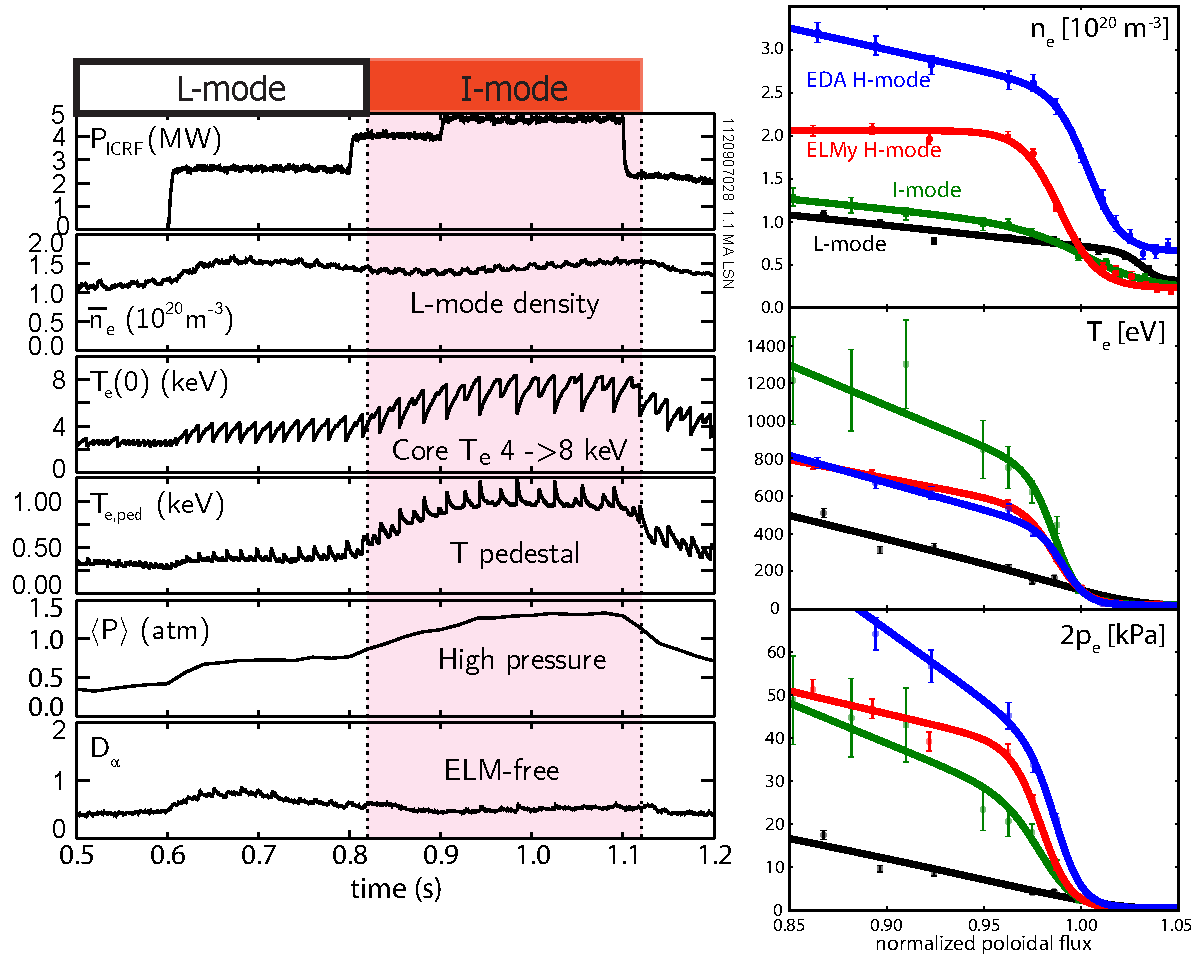
\includegraphics[width=\textwidth]{pdfgraphics/trace_imode.pdf}
 \caption{(left) characteristic time traces for an I-mode.  After the L-I transition, the core and edge temperature rise over several sawtooth cycles (visible in the oscillations in $T_e(0)$ and $T_{e,ped}$) before reaching a steady level; global pressure and confinement rise accordingly.  However, the density remains unchanged from the L-mode level.  No ELMs are exhibited on the $D_\alpha$ trace.  (right) pedestal profiles for L-, I-, and H-modes.  The I-mode (green) retains a density profile similar to L-mode (black), unlike the ELMy (red) and EDA (blue) H-modes, which form a strong density pedestal.  However, the I-mode forms a higher temperature pedestal than either H-mode, resulting in comparable pedestal pressures to H-mode while retaining L-mode particle transport.}
 \label{fig:imode_trace}
\end{figure}

Good progress has been made in understanding the pedestal structure and stability in I-mode \cite{Walk2014,Walk2014b}, particularly regarding the pedestal response to engineering inputs and stability against the MHD triggers associated with the ELM.
However, the development of I-mode as a viable reactor regime requires further understanding of the access and extrapolation of the mode to larger tokamak experiments, and its potential for desirable levels of performance on those devices.
In this paper, we first review the the responses of pedestal and core profiles (Section~\ref{sec:profiles}), and their impact on normalized performance (\eg volume-averaged $\beta_N$) and confinement.
Second, following the practices of the ITER89 \cite{Christiansen1992,Yushmanov1990} and ITER98 \cite{ITER1999} exercises, we establish an initial assay into a new confinement scaling for I-mode (Section~\ref{sec:scalings}) encompassing C-Mod data, with connections to empirical observation.
Lastly, we examine possible size dependences for the energy confinement, and subsequent extrapolations to larger devices (Section~\ref{sec:extrap}).

\note{add intro section on I-mode access?}

\section{Profiles and Responses}\label{sec:profiles}

\subsection{Pedestal Profiles}\label{subsec:ped}

A firm understanding of the pedestal is necessary for the establishment of the I-mode as a viable reactor regime.
To this end, a series of dedicated experiments \cite{Walk2014,Walk2014b} was conducted to examine the pedestal structure and stability in I-mode.
A scan of plasma current from $0.85$ to $1.35\;\mbox{MA}$ in a reversed-field, lower-null shape reveals a strong positive trend of pedestal electron temperature with current (Fig.~\ref{fig:Ip_Te95}) with the I-mode pedestal $T_e$ (for this paper, we use the pedestal parameters evaluated at the 95\% flux surface) meeting or exceeding H-mode levels at comparable plasma current.  

\begin{figure}[ht]
 \centering
 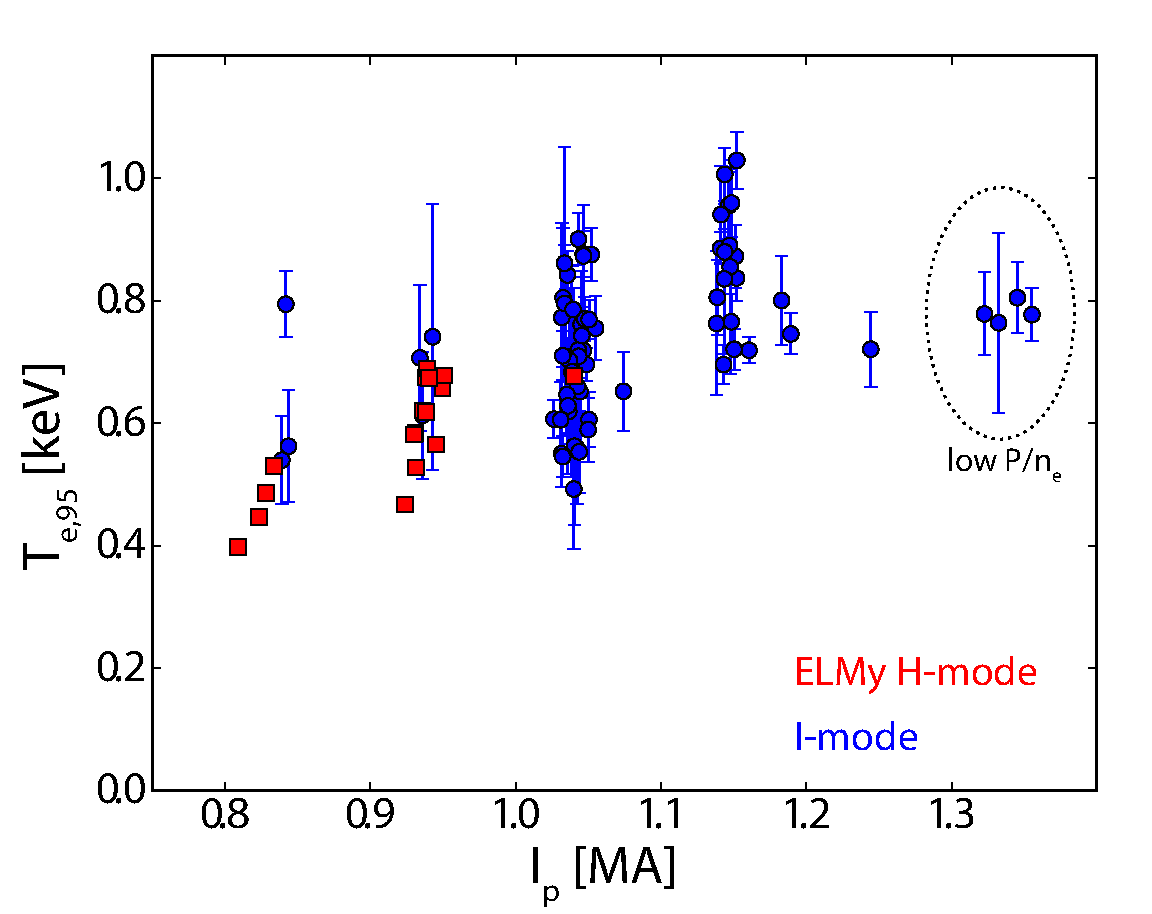
\includegraphics[width=0.75\textwidth]{Ip_Te95.pdf}
 \caption{Pedestal temperature versus plasma current, comparing ELMy H-modes and I-modes.  Notably, I-mode pedestal temperatures meet or exceed H-mode levels at comparable temperature, and trend positively with plasma current.  The spread at fixed current is due to varying power per particle (see Fig.~\ref{fig:Pnebar_Te95})}
 \label{fig:Ip_Te95}
\end{figure}

However, there is significant spread at fixed $I_p$, due to the wide variation in input heating power.
Examining a single current slice (Fig.~\ref{fig:Pnebar_Te95}) at $1.15\;\mbox{MA}$, we see a strong dependence of the pedestal temperature on net heating power, $P_{net} = P_{ICRF} + P_{Ohm} - P_{rad} - dW/dt$, normalized to the density (effectively, input heating power per particle).

\begin{figure}[ht]
 \centering
 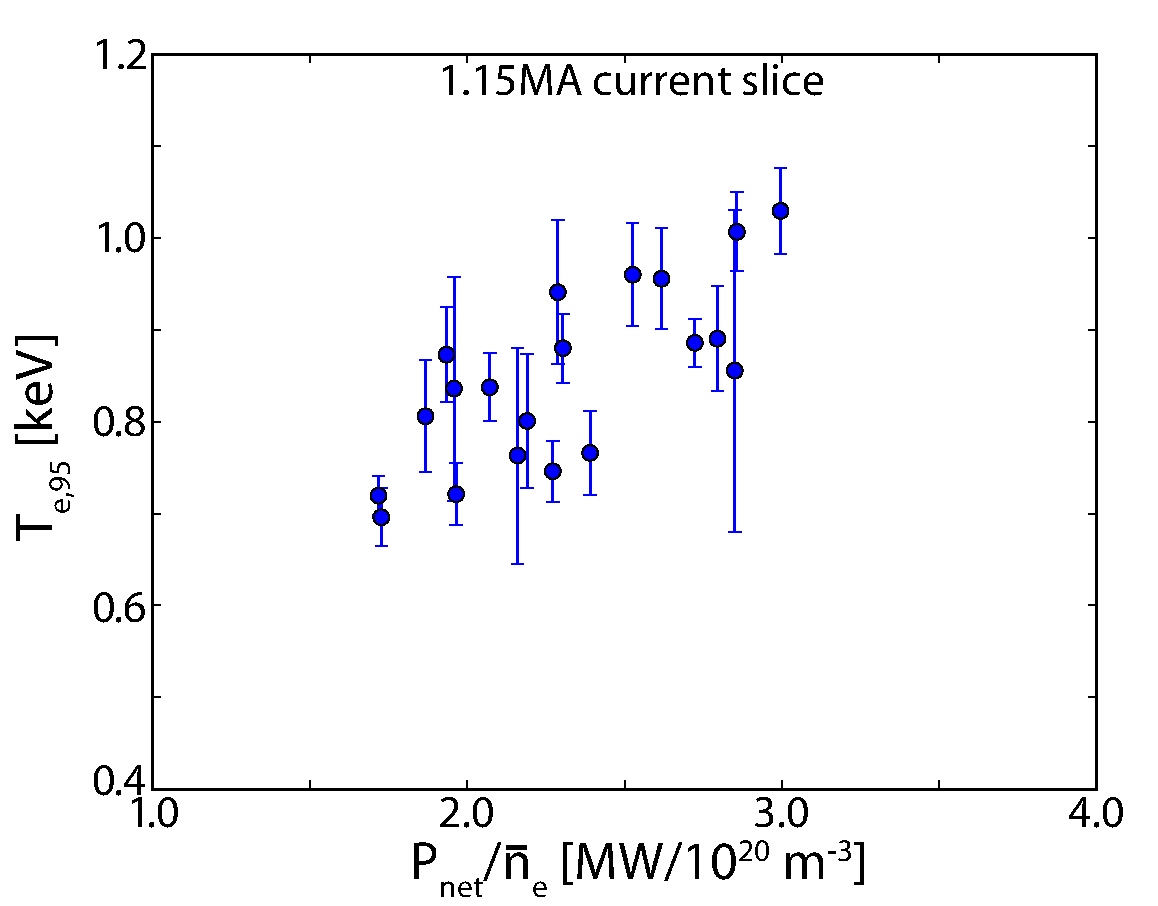
\includegraphics[width=0.75\textwidth]{Pnebar_Te95_115MA.pdf}
 \caption{Pedestal temperature versus heating power normalized to average density -- effectively, power per particle -- at $I_p = 1.15\;\mbox{MA}$, illustrating an approximate linear trend of the pedestal $T_e$ with $P_{net}/\overline{n}_e$ ($P_{net} = P_{ICRF} + P_{Ohm} - P_{rad} - dW/dt$)}
 \label{fig:Pnebar_Te95}
\end{figure}

In contrast to the temperature pedestal, the L-mode-like density profile in I-mode is set primarily through operator fueling via gas puffing.
Given sufficient heating power, temperature pedestals can be maintained alongside increased fueling across a broad range.
Example discharges matched in current, field, and shaping are shown in Fig.~\ref{fig:fuelingprofiles}, spanning a range in fueling and heating power, $\overline{n}_e = 1.0-1.7\times10^{20} \;\mbox{m}^{-3}$, $P_{net} = 2.75-4.10\;\mbox{MW}$.  
Temperature pedestals are matched across all three discharges despite the variation in fueling levels and edge densities, using consistent power per particle, $P_{net}/\overline{n}_e = 2.4-2.7\;\mbox{MW}/10^{20}\mbox{m}^{-3}$.

\begin{figure}[ht]
 \centering
 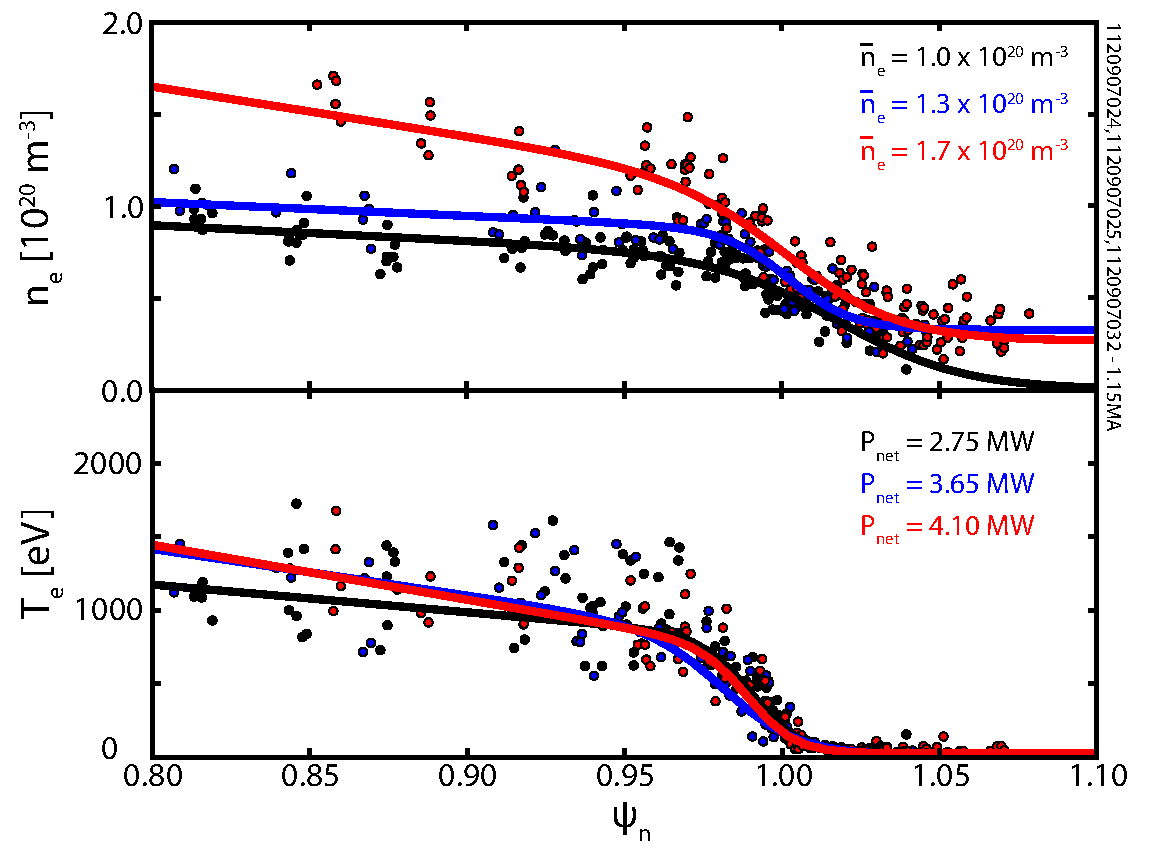
\includegraphics[width=0.75\textwidth]{fuelingprofiles.pdf}
 \caption{Three discharges, matched in current ($1.1\;\mbox{MA}$), field ($5.6\;\mbox{T}$), and shaping, fueled to $\overline{n}_e = 1.0, 1.3, 1.7 \times 10^{20} \;\mbox{m}^{-3}$, spanning a large fraction of the density range in the I-mode discharges presented here.  With sufficient heating power ($2.75, 3.65, 4.10 \;\mbox{MW}$), temperature pedestals can be matched across the fueling range.  This corresponds to power-per-particle values of $P_{net}/\overline{n}_e \sim 2.4-2.7 \;\mbox{MW}/10^{20}\mbox{m}^{-3}$.}
 \label{fig:fuelingprofiles}
\end{figure}

This behavior is distinct from that found in H-modes on C-Mod -- ELMy H-modes are limited, to good approximation, at a fixed pedestal $\beta_p$ determined by shaping, driving an inverse relationship between pedestal $n_e$ and $T_e$ at a given current, while transport-limited EDA H-modes lack operator control of the pedestal density at a given plasma current.
Independent control of the pedestal density and temperature profiles allows optimization of the energy confinement, fueling, and impurity venting for improved performance.
The pedestal $\beta_p$ and global performance may be strongly improved via matched increases in fueling and heating power (maintaining the target $P_{net}/\overline{n}_e$ for the temperature pedestal) after accessing the regime at lower power and density \note{access for ITER?}

\note{add pedestal pressure vs Wmhd?}

\subsection{Core Profiles}\label{subsec:core}

The high pedestal temperature in I-mode, coupled with core profile stiffness (such that higher temperatures supports a steeper marginally-stable $\nabla T_e$), supports very high core temperatures \note{add I-mode $T_e$ stiffness}.
With a moderate degree of core density peaking (with typical values of $n_{e0}/\langle n_e \rangle \sim 1.1-1.3$, comparable to H-mode) \note{add density peaking}, this supports comparable core and volume-averaged pressures to H-mode despite the comparatively relaxed pressure pedestal, supporting beneficial fusion conditions in the core while avoiding stability issues in the pedestal.  Example density, temperature, and pressure profiles for I-mode and H-mode are shown in Fig.~\ref{fig:coreprof}, illustrating the high core pressure attainable in I-mode despite the relaxed pedestal and lower density.

\begin{figure}[ht]
 \centering
 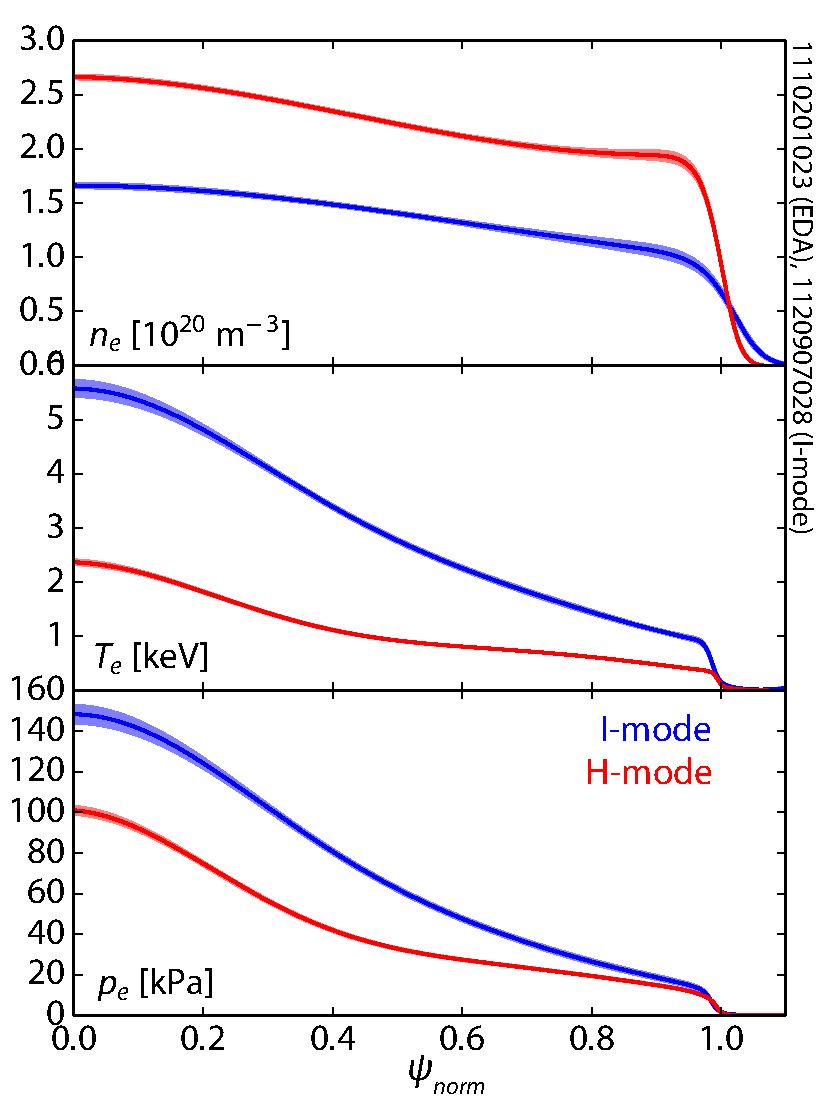
\includegraphics[width=0.75\textwidth]{coreprof_v3.pdf}
 \caption{Profiles in electron density, temperature, and pressure for I-mode and EDA H-mode, with $\pm \sigma$ errorbars indicated by the shaded region.  The H-mode case exhibits a very strong density pedestal, with a somewhat reduced temperature pedestal; the I-mode, in contrast, has a significant temperature pedestal with a relaxed density profile.  While this typically results in a reduced pedestal pressure in I-mode compared to H-mode, core profile stiffness supports very high central temperatures, such that I-mode exhibits comparable or greater core and average pressure despite the relaxed pedestal.}
 \label{fig:coreprof}
\end{figure}

Accordingly, I-modes on C-Mod inhabit a comparable range in global confinement metrics, as shown in Fig.~\ref{fig:betan_H}.  In both global normalized beta ($\langle \beta_N \rangle = \langle \beta \rangle aB_T/I_p$) and normalized confinement $H_{98}$, the I-mode occupies a comparable range to ELMy H-mode, indicating competitive levels of global confinement while maintaining desirable ELM stability and impurity confinement behaviors.

\begin{figure}[ht]
 \centering
 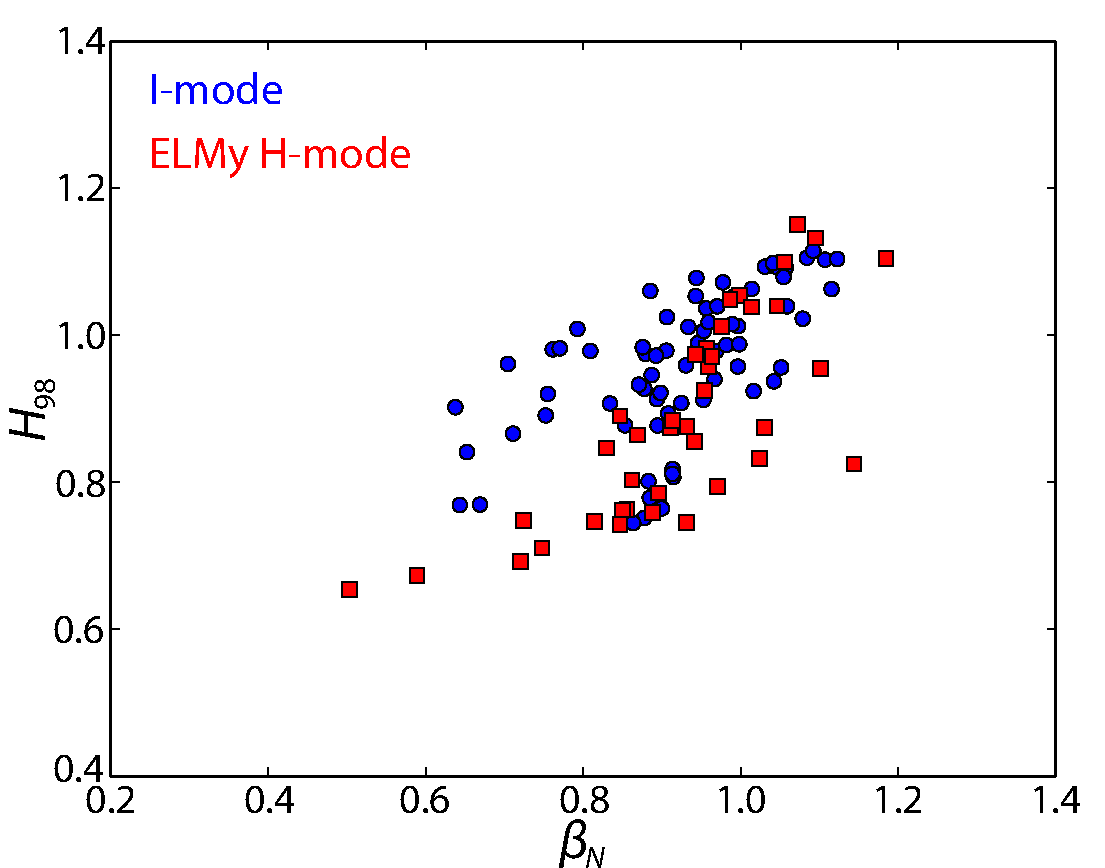
\includegraphics[width=0.75\textwidth]{betan_H_i_e.pdf}
 \caption{Global normalizezd $\beta_N$ versus confinement factor $H_{98}$ for I-mode and ELMy H-mode.  Despite the relaxed pedestal pressure, I-modes reach comparable average pressures, while maintaining H-mode-like energy confinement.}
 \label{fig:betan_H}
\end{figure}

\section{I-Mode Confinement Scalings}\label{sec:scalings}

Due to the complexities inherent in the processes responsible for energy trasport -- both short-wavelength drift-wave turbulence and longer-wavelength MHD processes -- it is difficult to model energy confinement from first principles.
Rather, it is common to establish empirical scaling laws for energy confinement using a power-law fit to large datasets.
For example, the ITER89 \cite{Yushmanov1990} and ITER98 \cite{ITER1999} exercises utilized an extensive multi-machine database \cite{Christiansen1992} for L-mode and ELMy H-mode confinement respectively.
In particular, the ITER98y2 scaling is used as a common baseline for performance in high-confinement regimes, particularly in terms of its normalized factor $H_{98}$ \note{define this?  earlier?}

While the $H_{98}$ factor is commonly used as a figure of merit for high-performance regimes (particularly, ELM-suppressed H-modes developed more recently than the ITER98 scaling exercise), it is, effectively, simply a measurement of the quality of the ITER98 prediction to the data.
As the ITER98 scaling was constructed using predominantly ELMy H-modes, it implicitly includes the physics of ELM-limited pedestals -- for confinement regimes governed by substantially different physics, this is not necessarily a good prediction.
While I-mode data is currently largely limited to C-Mod, and is insufficient for a full confinement scaling (particularly, to develop the dependence on machine size), it is nonetheless illustrative to examine a dedicated I-mode confinement scaling.

I-mode energy confinement times are fitted in an ordinary least-squares sense to an ITER98-like power law of the form

\begin{equation}
 \tau_{I-mode} = C \; I_p^{\alpha_{I_p}} \; B_T^{\alpha_{B_T}} \; \overline{n}_e^{\alpha_{n_e}} \; R^{\alpha_R} \; \varepsilon^{\alpha_\varepsilon} \; \kappa^{\alpha_\kappa} \; P_{loss}^{\alpha_P}
\end{equation}

\noindent to find free exponents $\alpha_j$ for plasma current $I_p$ in MA, toroidal field $B_T$ in T, line-averaged density $\overline{n}_e$ in $10^{20}\;\mbox{m}^{-3}$, major radius $R$ in m, inverse aspect ratio $\varepsilon$, elongation $\kappa$, and loss power $P_{loss} = P_{Ohm} + P_{ICRF} - dW/dt$ in MW.
Although the net power $P_{net}$ has been demonstrated to be the more suitable parameter, rather than $P_{loss}$ \cite{Hughes2002}, we use $P_{loss}$ here for consistency with previous scaling exercises, and to enable the use of older I-mode data without consistent measurements of the radiated power.
However, the radiated power is typically a small fraction of the total power in I-mode ($P_{rad} < 900\;\mbox{kW}$, $P_{rad}/P_{tot} < 20\%$), so this is sufficient for an initial assessment of the confinement.

Results from the fitting exercise are shown in Table~\ref{tab:fits}, containing the values and standard deviations for each exponent, the scale factor $C$, and the $r^2$ coefficient of determination for the fit.
Fit (a) in the table uses the full parameter list used in the ITER98y2 scaling \note{figure?}.
However, it is immediately obvious that the size scalings, dependent on major radius $R$ and aspect ratio $\varepsilon$, are not properly captured (denoted by the extreme errorbars on these exponents).
This is to be expected -- absent meaningful variation in $R$ and $\varepsilon$ in the dataset (which requires multiple machines to produce) these parameters are not well-constrained, and result (a) is over-fitted.
These parameters are omitted in result (b), yielding a minimum-complexity fit on $I_p$, $B_T$, $\overline{n}_e$, and $P_{loss}$.
The results of this fit are shown in Figure~\ref{fig:taue_cmod}, with the data distinguished between older reversed-field LSN and forward-field USN discharges, as well as a newer dedicated pedestal profile database \cite{Walk2014}.

\begin{table}[ht]
 \centering
 \begin{tabular}{ccc}
  \hline
  $\alpha_j$ & (a) & (b)\\
  \hline
  $C$ & $0.040 \pm 0.066$ & $0.014 \pm 0.002$ \\
 $I_p$ & $0.686 \pm 0.074$ & $0.685 \pm 0.076$ \\
  $B_T$ & $0.698 \pm 0.075$ & $0.768 \pm 0.072$ \\
  $\overline{n}_e$ & $-0.077 \pm 0.055$ & $0.017 \pm 0.048$ \\
  $R$ & $4.219 \pm 4.623$ & \\
  $\varepsilon$ & $0.127 \pm 1.144$ & \\
  $\kappa$ & $1.686 \pm 0.398$ & \\
  $P_{loss}$ & $-0.197 \pm 0.048$ & $-0.286 \pm 0.042$ \\
  $r^2$ & $0.713$ & $0.685$ \\
  \hline
 \end{tabular}
 \caption{Parameters for the power-law scalings for I-mode energy confinement time $\tau_E$, along with $r^2$ coefficients of determination for the fit.  The full ITER98-like fit (a) is over-constrained, lacking sufficient range in the data to fit $R$, $\varepsilon$, and $\kappa$.  These parameters are omitted in the minimum-complexity fit (b).  Parameters are in the given units: $I_p$ in MA, $B_T$ in T, $\overline{n}_e$ in $10^{20}\;\mbox{m}^{-3}$, $R$ in m, and $P_{loss}$ in MW.  Elongation $\kappa$ and inverse aspect ratio $\varepsilon$ are dimensionless.}
 \label{tab:fits}
\end{table}

\begin{figure}[ht]
 \centering
 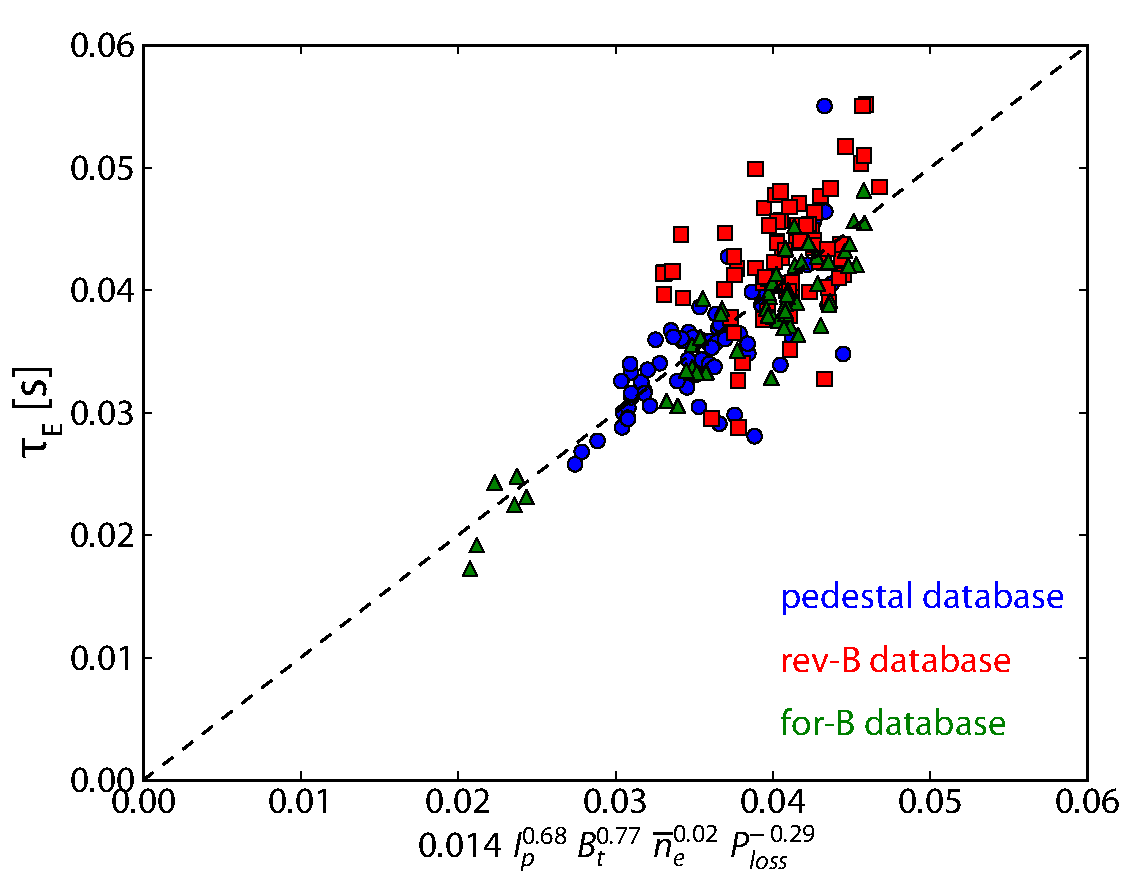
\includegraphics[width=0.75\textwidth]{tauE_3_Ploss_sep.pdf}
 \caption{C-Mod I-mode data from older reversed-field and forward-field databases, as well as the newer dedicated pedestal database, showing measured energy confinement time $\tau_E$ versus the minimum-complexity fit from Table~\ref{tab:fits}.  $R^2$ coefficient of determination for the fit is $0.685$.}
 \label{fig:taue_cmod}
\end{figure}

A comparison of the results from the minimum-complexity I-mode fit against the corresponding parameters from the ITER89 and ITER98y2 scalings is shown in Table~\ref{tab:compare}.  
Notably, the I-mode fit exhibits a much stronger dependence on magnetic field, and weaker degradation of the confinement with heating power, compared to either the L-mode or H-mode fits.
This is consistent with the observed behavior in I-mode, both on C-Mod and elsewhere.
The threshold power for the transition to H-mode (which brackets the upper range of the I-mode operational window) typically is strongly elevated with increasing magnetic field \cite{Martin2008}; however, the L-I threshold does not meaningfully vary with magnetic field.
Thus, the increased magnetic field broadens the operational window for I-mode, as shown in Figure~\ref{fig:Bt_P}.
The strong dependence of the confinement on $B_T$ may be explained by the more aggressive pedestals possible at higher field while avoiding the H-mode transition.
Similarly, the weak power degradation in the I-mode $\tau_E$ is reflected in experimental observations of the plasma stored energy in relation to the plasma current and heating power (Figure~\ref{fig:PIp_W}).

\begin{table}[ht]
 \centering
 \begin{tabular}{ccccc}
  \hline
  $\alpha_j$ & ITER89 & ITER98y2 & I-mode & \\
  \hline
  $I_p$ & 0.85 & 0.93 & 0.69 & \\
  $B_T$ & 0.2 & 0.15 & \textcolor{red}{0.77} & \small{\textcolor{red}{much stronger field dependence}}\\
  $\overline{n}_e$ & 0.1 & 0.41 & 0.02 & \\
  $P_{loss}$ & -0.5 & -0.69 & \textcolor{red}{-0.29} & \small{\textcolor{red}{weak power degradation}} \\
  $R$ & 1.5 & 2 &  & \small{need other machine input} \\
  $\varepsilon$ & 0.3 & 0.5 &  & \\
  $\kappa$ & 0.5 & 0.78 &  & \\
  \hline
 \end{tabular}
 \caption{Comparison of power-law exponents for the ITER89 and ITER98y2 fits, and the minimum-complexity I-mode fit.  In particular, the I-mode fit exhibits a much stronger dependence on toroidal field, and weaker degradation with input heating power.}
 \label{tab:compare}
\end{table}

\begin{figure}[ht]
 \centering
 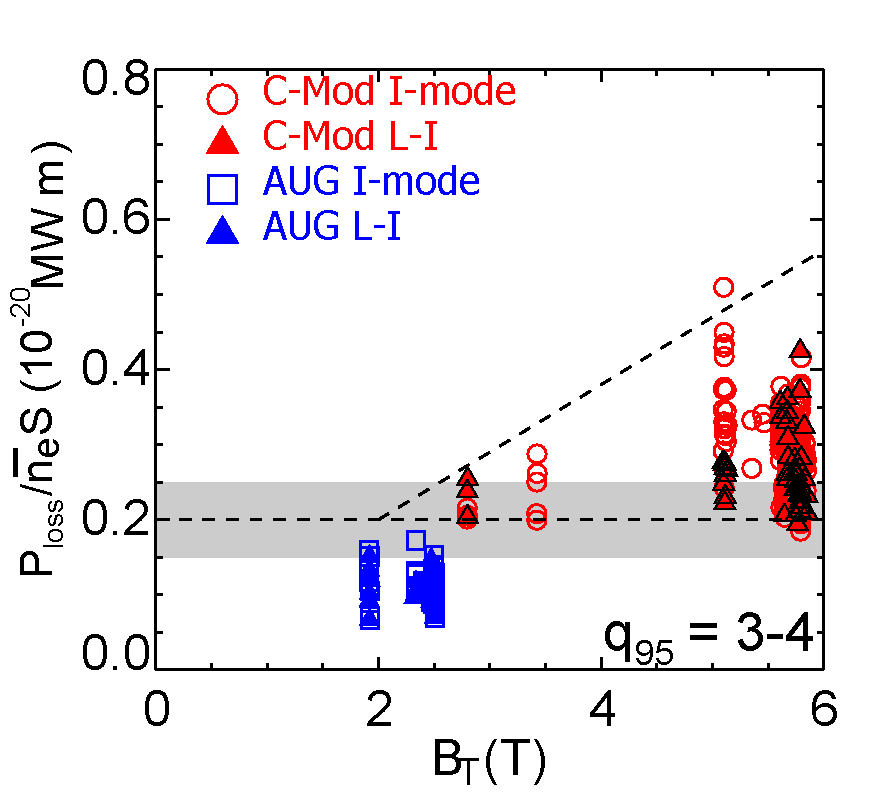
\includegraphics[width=0.75\textwidth]{Bt_Pthres_Cmod_AUG.pdf}
 \caption{\note{work out caption with Amanda?}}
 \label{fig:Bt_P}
\end{figure}

\begin{figure}[ht]
 \centering
 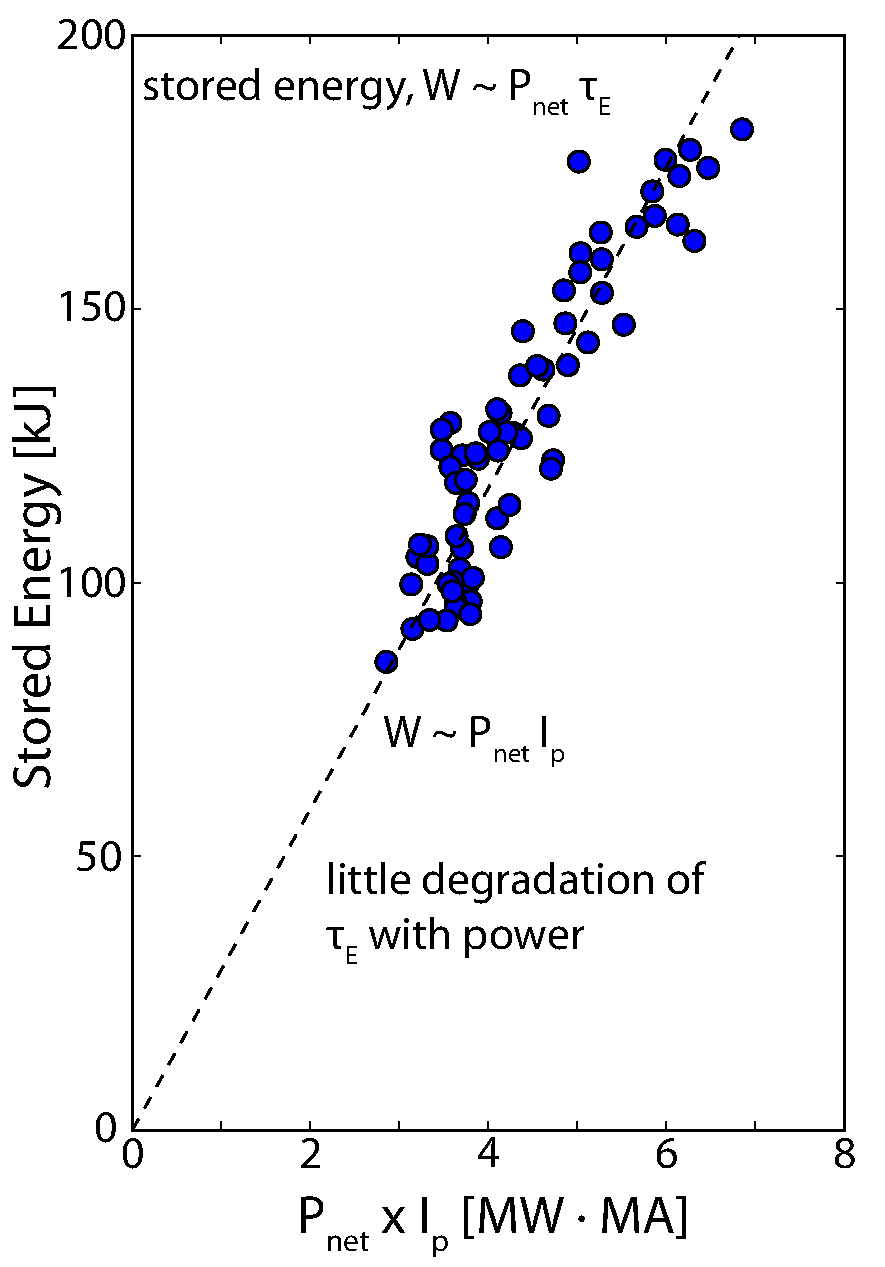
\includegraphics[width=0.75\textwidth]{PIp_W_scale.pdf}
 \caption{I-mode stored energy versus the product of net heating power $P_{net}$ and plasma current $I_p$.  Based on the H-mode confinement scaling, $\tau_E$ is expected to scale linearly with $I_p$, and to show a strong degradation with heating power, $\tau_E \sim I_p \times P^{-0.7}$.  As the stored energy is given by $W \sim P \tau_E$, this should yield $W \sim I_p P_{net}^{0.3}$.  The observed linear trend is consistent with little degradation of $\tau_E$ in I-mode with heating power. \note{exchange for fixed-current version?}}
 \label{fig:PIp_W}
\end{figure}

\subsection{Normalized Confinement}\label{subsec:norm}

We may define a normalized confinement factor

\begin{figure}[ht]
 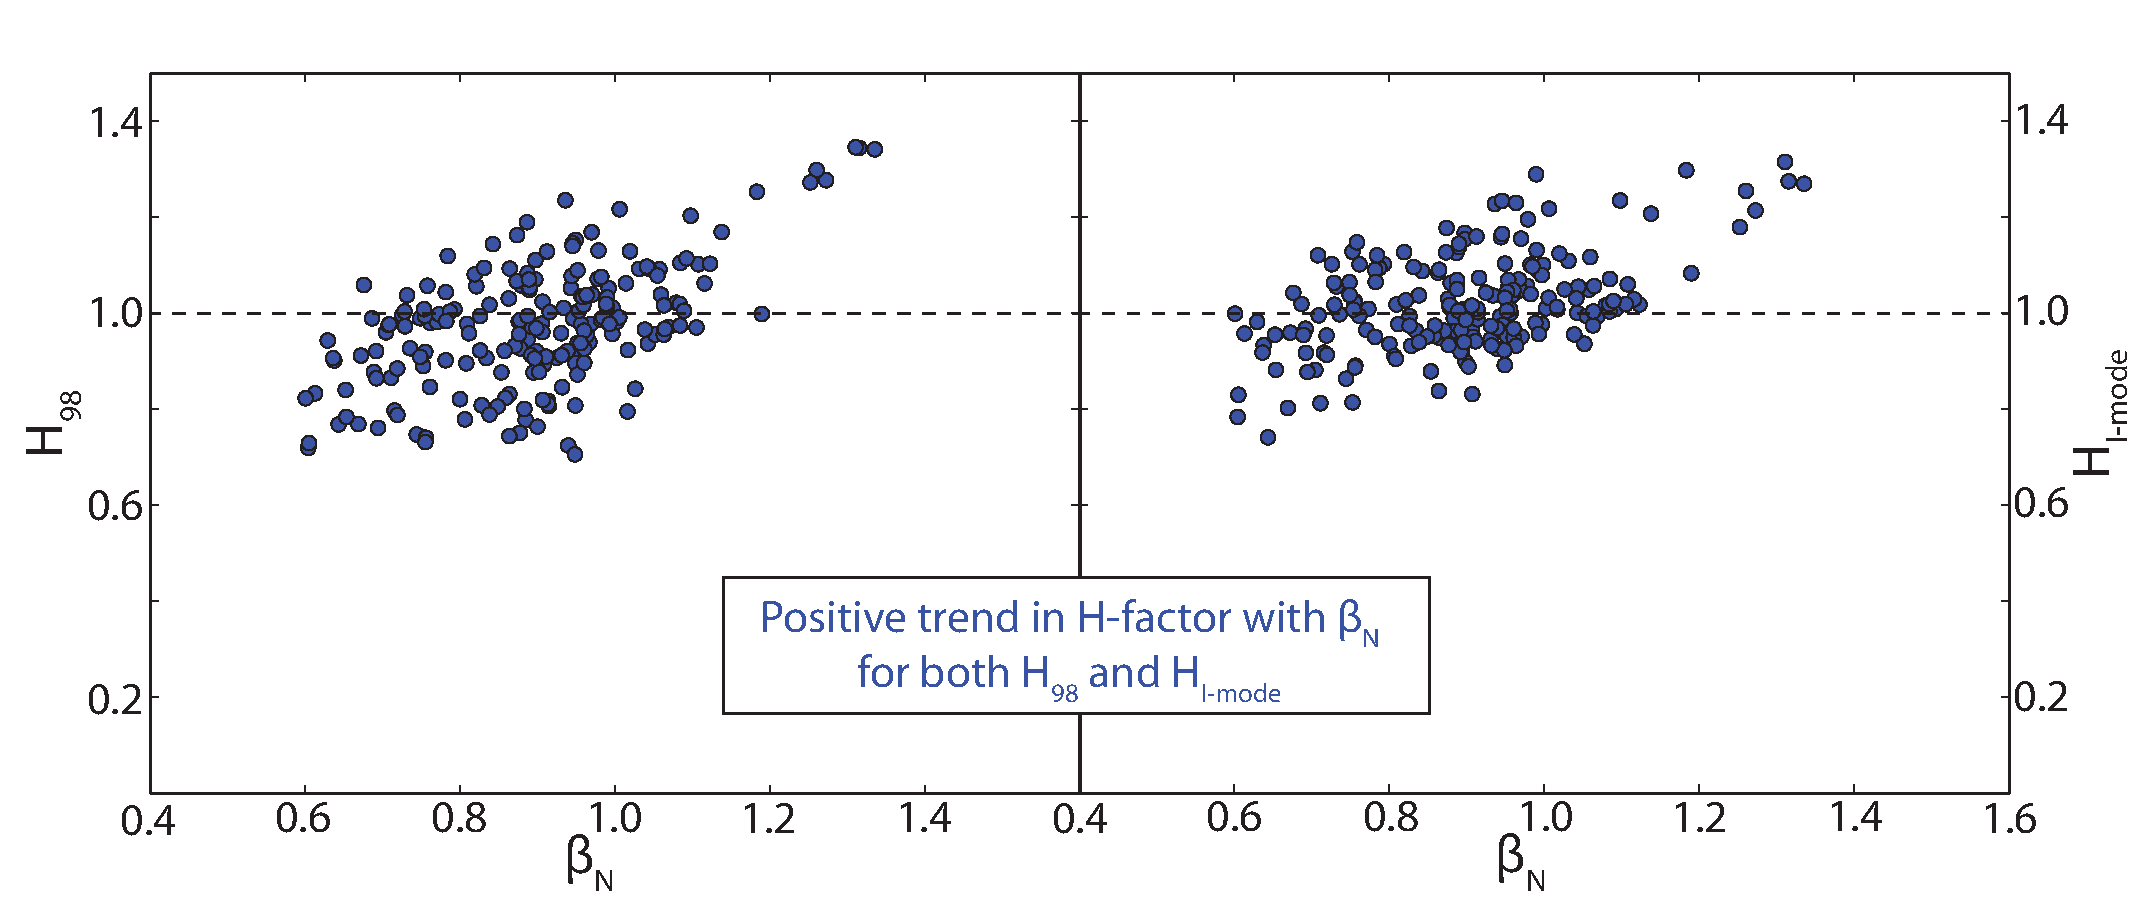
\includegraphics[width=\textwidth]{betaN_H.pdf}
 \caption{Confinement normalized to the ITER98y2 (left) and I-mode (right) scalings, versus volume-average $\beta_N$.  In both, a positive trend of normalized confinement with beta is observed, consistent with observations in H-mode.}
 \label{fig:betaN_H}
\end{figure}

\begin{figure}[ht]
 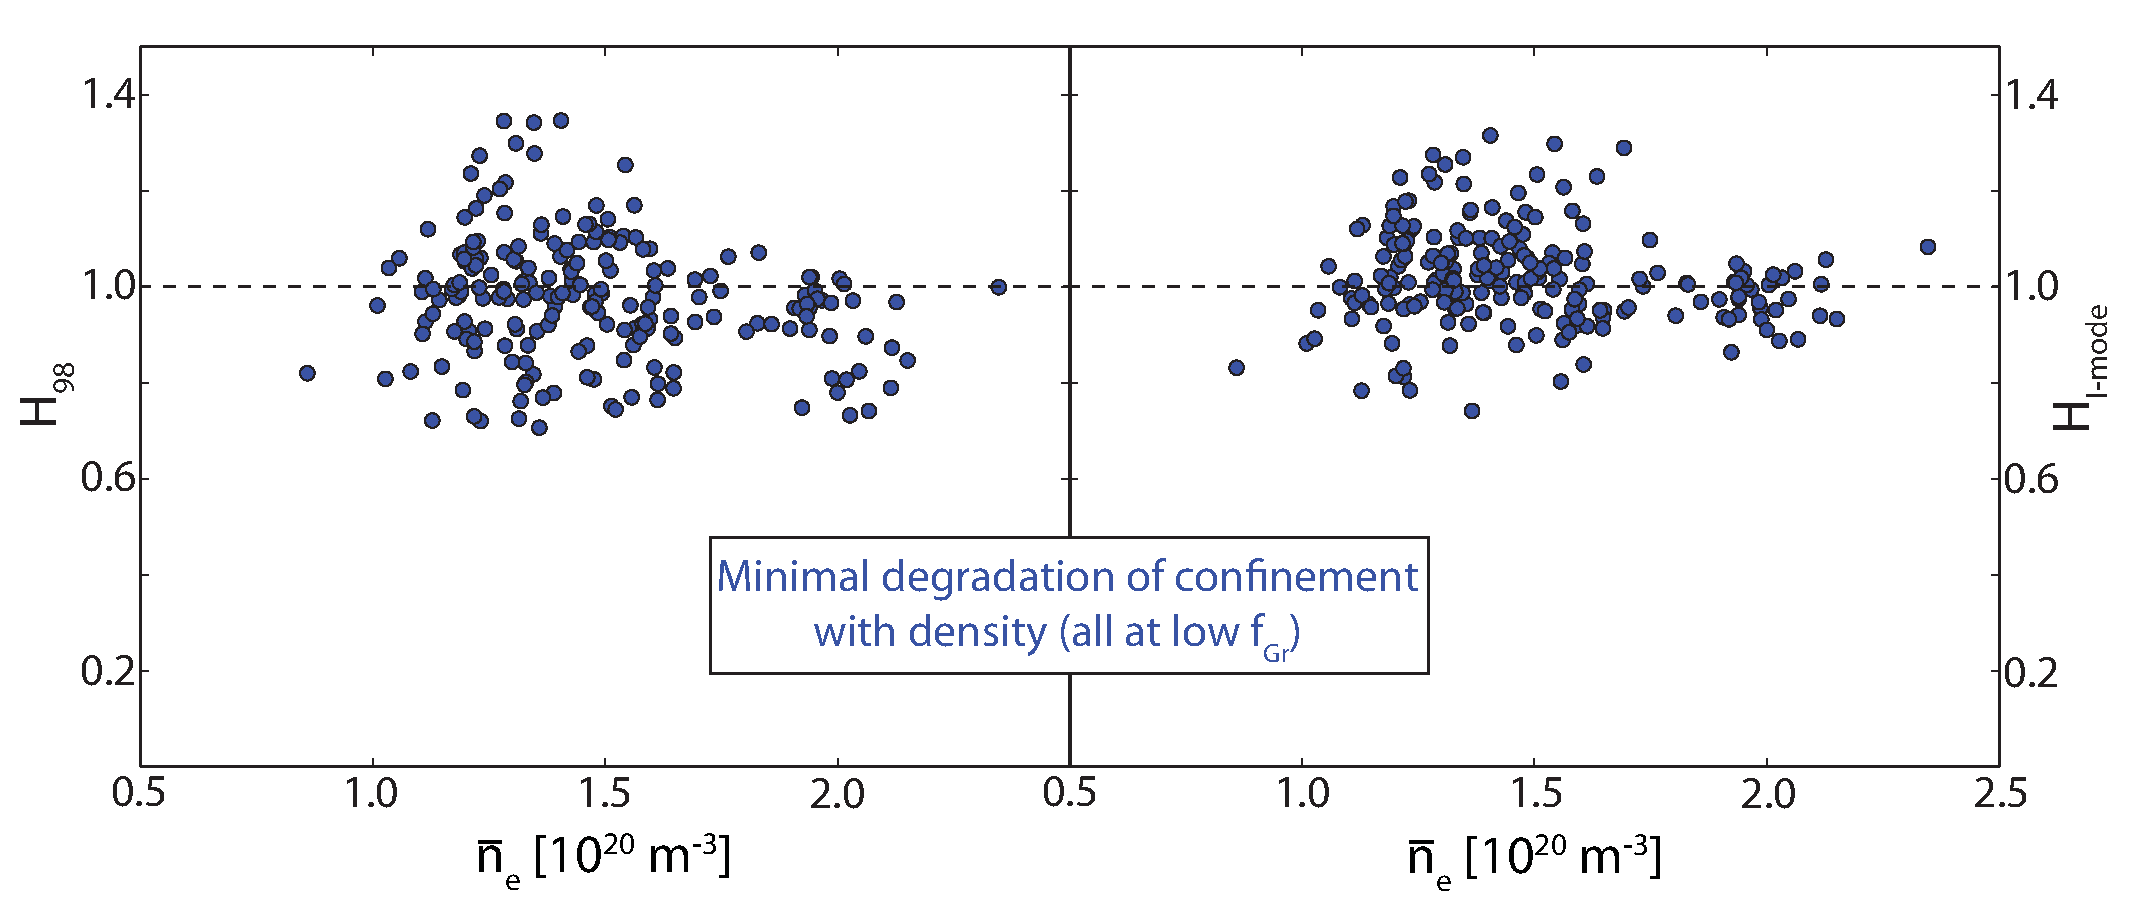
\includegraphics[width=\textwidth]{nebar_H.pdf}
 \caption{Confinement normalized to the ITER98y2 (left) and I-mode (right) scalings, versus line-averaged density $\overline{n}_e$.  Neither case shows significant degradation of confinement with density (unlike H-mode) although the highest normalized-confinement cases do occur at lower density (largely due to the lower radiated-power fraction in these cases).}
 \label{fig:nebar_H}
\end{figure}

\subsection{Covariances}\label{subsec:covar}

\section{Extrapolation to Larger Devices}\label{sec:extrap}

\section{Conclusions}\label{sec:conclusion}

\section*{References}
\bibliographystyle{unsrt}
\bibliography{jrwalk_references}

\end{document}